\chapter{Re\c{t}elele neuronale}

\section{Neuronul}

Re\c{t}elele Neuronale au pornit de la ideea de a crea un model matematic care s\u{a} imite structura \c{s}i comportamentul unui creier uman.
\par
Creierul este compus din mai multe unit\u{a}\c{t}i numi\c{t}i neuroni, care comunic\u{a} \^{i}ntre ei prin sinapse, se aproximeaz\u{a} faptul c\u{a} creierul uman are aproximativ 86 de miliarde de neuroni \c{s}i 10^{14} - 10^{15}  sinapse.


\includegraphics[width=300]{neuron_small.png}

Fiecare neuron prime\c{s}te impulsuri prin dedridele sale de la al\c{t}i neuroni \c{s}i produce impulsuri prin axon pe care il transmite mai departe la al\c{t}i neuroni prin sinapse.

\par

Acest model biologic a incercat sa fie imitat de c\u{a}tre Warren McCulloch \c{s}i Walter Pitts \^{i}n anul 1943, astfle \^{i}ncat ace\c{s}tia au creat un model matematic care s\u{a} semene c\^{a}t mai mult cu varianta biologic\u{a}. \^{I}n modelul matematic propus de ace\c{s}tia datele de intrare primite prin dendrive ( s\u{a} le not\u{a}m cu \textbf{\textit{x}} ) sunt multiplicate cu ni\c{s}te \^{i}nt\u{a}riri ( s\u{a} le not\u{a}m cu \textbf{\textit{W}} ) pentru a se imita transferul facut prin sinapse \^{i}ntre axonul neuronului care transmite datle \c{s}i dendrivele neuronului care prime\c{s}te datele. Corpul neuronului a devenit un sumator care \^{i}nsumeaza produsul primit de la dendrive, astfel c\u{a} acesta se poate definii prin urm\u{a}toarea formul\u{a}  $$ \sum_{i=1}^{n} W_i x_i $$ unde \textbf{\textit{n}} reprezint\u{a} num\u{a}rul de dendrive. La aceast\u{a} formul\u{a} se mai insumeaz\u{a} un \textit{biases} ( s\u{a} \^{i}l not\u{a}m cu \textbf{\textit{b}} ) pentru a reprezenta caracteristicile neliniare ale neuronului. Cu aceast\u{a} nou\u{a} \^{i}nsumare formula va devenii $$ \sum_{i=1}^{n} W_i x_i + b $$
Dac\u{a} rezultatul ob\c{t}inut este mai mare dec\^{a}t un prag acesta va trece mai departe prin axon spre al\c{t}i neuroni. S\u{a} definim acest efect printr-o func\c{t}ie \textbf{\textit{f}} pe care o vom numii \textit{func\c{t}ie de activare} care stabile\c{s}te dac\u{a} un semnal trece mai departe sau nu, vom descrie mai pe larg aceast\u{a} func\c{t}ie in capitolele de mai jos, astfel c\u{a} modelul matematic a neuronului se poate rezuma la urm\u{a}toarea formul\u{a} 
$$f( \sum_{i=1}^{n} W_i x_i + b ) $$

\par

Trebuie precizat faptul c\u{a} modelul matematic al neuronului prezentat mai sus nici mac\u{a} nu se apropie de adevaratul comportament al unui neuron, acesta din urm\u{a} av\^{a}nd \^{i}n creierul uman un rol mult prea complex pentru a putea fi exprimat printr-o simpl\u{a} func\c{t}ie. 


\section{Fun\c{t}ia de activare}

A\c{s}a cum am specificat \c{s}i mai sus, o re\c{t}ea neuronala are nevoie de o fun\c{t}ie de activare care s\u{a} decid\u{a} dac\u{a} datele pot trece mai departe la urmatorii neuroni sau nu. De-a lungu istoriei s-au folosit mai multe tipuri de fun\c{t}ii de activare la re\c{t}elele neuronale, \^{i}nsa cea care d\u{a} cel mai bun randament at\^{a}t la timpul de antrenare c\^{a}t \c{s}i la acurate\c{t}ea final\u{a} este func\c{t}ia de activare ReLU (Rectified Linear Unit).

\subsection{Rectified Linear Unit}

Rectified Linear Unit, sau mai pe scurt ReLU, este la ora actual\u{a} cea mai folosit\u{a} fun\c{t}ie de activare, ea av\^{a}nd urm\u{a}toarea formul\u{a}

\[ f(x) =
  \begin{cases}
    0       & \quad \text{dac\u{a} } x \leq 0\\
    x  & \quad \text{dac\u{a} } x > 0\\
  \end{cases}
\]

Cu alte cuvinte func\c{t}ia pur \c{s}i simplu nu las\u{a} s\u{a} treac\u{a} mai departe rezultatele negative in urma efectu\u{a}rii opera\c{t}iilor din corpul neuronului.

\section{Arhitectura unei re\c{t}ele neuronale}

Acum c\u{a} am aflat ce este un neuron \c{s}i cum este simulat acesta din punct de vedere matematic trebuie s\u{a} discut\u{a}m cum sunt structura\c{t}i ace\c{s}tia \^{i}ntr-o re\c{t}ea neuronal\u{a}, pentru c\u{a} o re\c{t}ea nuronal\u{a} este compus\u{a} din milioane sau chiar sute de milioane de neuroni iar structurarea acestora este foarte important\u{a}.

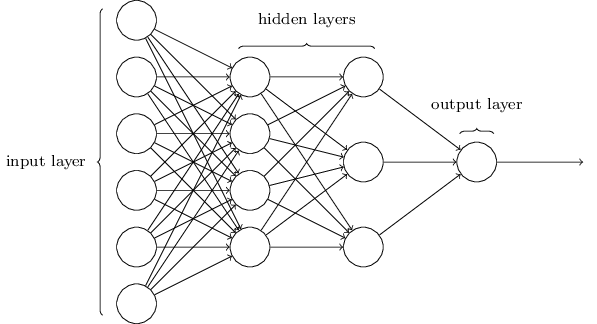
\includegraphics[width=300]{image10.png}

Re\c{t}elele neuronale sunt modelate ca o cole\c{t}ie de neuroni pe nivele, unde datele calculate de un nivel devin datele de intrare pentru urmatorul nivel de neuroni. Dupa cum se vede \c{s}i in imaginea de mai sus, neuronii afla\c{t}i pe acela\c{s}i nivel nu comunic\u{a} direct unii cu ceilal\c{t}i, comunicarea realiz\^{a}nduse doar cu nivelul inferior de neuroni \c{s}i cu nivelul superior de neuroni.
\par
Primul nivel al unei re\c{t}ele neuronale se nume\c{s}te nivelu input, deoarece acesta reprezint\u{a} doar date de intrare, iar ultimul nivel al unei re\c{t}ele neuronale se nume\c{s}te nivelul output, doarece acesta intoarce valoarea final\u{a}, nivelele dintre primul \c{s}i ultimul nivel se numesc nivelele ascunse ( hidden layers ).
\par
Re\c{t}elele neuronale, ca cea de mai sus, se numesc re\c{t}ele feedforward, deoarece outputul unui nivel merge tot timpul la urm\u{a}torul nivel, nu se intoarce niciodat\u{a} la un nivel anterior.
\par 
Pentru a se in\c{t}elege mai bine cum lucreaz\u{a} o re\c{t}ea neuronal\u{a} vom nota cu \textbf{\textit{x}} datele de intrare de la nivelul input, cu \textbf{\textit{h}} fiecare hidden layer, cu \textbf{\textit{W}} \^{i}ntaririle, cu \textbf{\textit{b}} bias-ul si cu \textbf{\textit{f}} func\c{t}ia de activare, astfle c\u{a} modelul de mai sus cu dou\u{a} niveluri hidden se poate exprima prin urm\u{a}torul algoritm:

$$h_1 = f( \sum_{i=1}^{n} W_1_i x_i + b_1 ) $$
$$h_2 = f( \sum_{i=1}^{n} W_2_i h_1_i + b_2 ) $$
$$out = f( \sum_{i=1}^{n} W_3_i h_2_i + b_3 ) $$

\par

Unul dintre motivele pentru care re\c{t}elele neuronale sunt organizate pe nivele este acela c\u{a} pe acest timp de structur\u{a} este mai u\c{s}or s\u{a} se efectueze opera\c{t}ii pe matrici, astfel inc\^{a}t sa nu mai fim nevoi\c{t}i s\u{a} facem multiplic\u{a}ri individuale. Spre exemplu, s\u{a} lu\u{a}m un \textbf{\textit{x}} de dimeniusne [10x10], $W_1, W_2 $ \c{s}i $W_3$ de dimensiune [5x10], [3x5], respectiv [1x3], iar $b_1, b_2 $ \c{s}i $b_3$ de dimensiune [5x1], [3x1] \c{s}i [1x1], atunci algoritmul de mai sus se poate rescrie in felul urmator: 

$$h_1 = f( W_1 x + b_1 ) $$
$$h_2 = f( W_2 h_1 + b_2 ) $$
$$out = f( W_3 h_2 + b_3 ) $$

unde $h_1$ este de dimensiune [5x10], $h_2$ de dimensiune [3x10], iar out de dimensiune [1x10]. Parametrii $W_1, W_2, W_3, b_1, b_2, b_3$ sunt paramterii pe care re\c{t}eaua neuronal\u{a} \^{i}i inva\c{t}\u{a} pentru a atinge o accurate\c{t}e c\^{a}t mai mare. Despre procesul de inv\u{a}\c{t}are a parametrilor \c{s}i despre cum trebuie s\u{a} \^{i}i set\u{a}m la inceput vom discuta \^{i}n capitolele ce urmeaz\u{a}.

\section{Initializarea parametrilor}

Am v\u{a}zut mai sus cum s\u{a} construim o re\c{t}ea neuronal\u{a}. \^{I}nainte ca s\u{a} discut\u{a}m descpre cum se antreneaz\u{a} o re\c{t}ea neuronal\u{a} trebuie s\u{a} discumta cum ini\c{t}ializ\u{a}m cele dou\u{a} tipuri de parametrii (\^{i}nt\u{a}ririle \c{s}i bias - urile). 

\subsection{Initializarea \^{i}nt\u{a}ririlor}

Av\^{a}nd in vedere c\u{a} nu \c{s}tiim valorile finale pe care o s\u{a} le aibe \^{i}nt\u{a}ririle la finalul procesului de antrenare a re\c{t}elei neuronale, deoarece aceste valori se actualizeaz\u{a} la fiecare pas de antrenare, va trebuii s\u{a} ini\c{t}ializ\u{a}m \^{i}nt\u{a}ririle astfle \^{i}nc\^{a}t o jum\u{a}tate din valori s\u{a} aibe valori negative iar cealalt\u{a} jum\u{a}tate valori pozitive, vom dorii valori unice pentru fiecare \^{i}ntarire pentru a acoperii o gam\u{a} c\^{a}t mai larg\u{a} de valori posibile pentru \^{i}nt\u{a}riri iar acestea s\u{a} fiu c\^{a}t mai aproape de valorea zero dar diferite de zero astfle \^{i}nc\^{a}t s\u{a} fiu mai u\c{s}or de actualizat.

\par

Pentru a \^{i}ndeplinii condi\c{t}iile de mai sus vom folosii o distribu\c{t}ie normal\u{a} cu media zero \c{s}i cu devia\c{t}ia standard $\frac{1}{\sqrt{n}}$ , unde n reprezint\u{a} numarul de variabile pe care \^{i}nt\u{a}rirea o are. Acest lucru asigur\u{a} faptul c\u{a} toate \^{i}nt\u{a}ririle din re\c{t}eaua neuronal\u{a} au la inceput aceea\c{s}i distribu\c{t}ie de numere, lucru care va facilita antrenarea mai rapid\u{a} a re\c{t}elei neuronale.

\par 

Dup\u{a} cum \c{s}tiim, varian\c{t}a reprezint\u{a} media patratic\u{a} a abaterilor in m\u{a}rime absolut\u{a} a valorilor inregistrare fat\u{a} de media aritmetic\u{a} care ne spune c\^{a}t de mare este r\u{a}sp\^{a}ndirea  acestui set. Mai precis, varian\c{t}a m\u{a}soar\u{a} c\^{a}t de apropiate sunt valorile setului de date de valoarea medie a acestuia.

$$Var = \frac{1}{n} \sum_{i=1}^{n} (x_i - m )^2 $$

\^{I}n formula de mai sus m reprezint\u{a} media aritmetic\u{a} iar $x_i$ valaorile date. \^{I}n cazul nostru dorim ca varian\c{t}a datelor de intrare sa nu se schimbe dup\u{a} ce iese din neuron \c{s}i se duce spre func\c{t}ia de activare pentru a nu altera datele foarte tare de la un nivel la altul. \^{I}n acest caz

$$Var(\sum_{i=1}^{n} W_i x_i) = \sum_{i=1}^{n} Var(W_i x_i) = $$
$$ = \sum_{i=1}^{n} [E(W_i)]^2 Var(x_i) + [E(x_i)]^2 Var(W_i) + Var(x_i) Var(W_i)$$

Presupunem c\u{a} setul de date \c{s}i \^{i}nt\u{a}ririle au media zero \c{s}i sunt distribuite identic, astfel c\u{a} formula de mai sus se transform\u{a} \^{i}n

$$\sum_{i=1}^{n} Var(x_i) Var(W_i) = (n Var(W)) Var(x)$$

care trebuie sa fie egal\u{a} cu varian\c{t}a datelor de intrare, asta \^{i}nseamn\u{a} c\u{a} 

$$n Var(W) = 1 \implies Var(W) =  \frac{1}{n} $$

\c{s}i \c{t}in\^{a}nd cont c\u{a} varian\c{t}a unei distribu\c{t}ii normale este p\u{a}tratul devia\c{t}iei standard, atunci rezult\u{a} c\u{a} devia\c{t}ia standard are valoarea $\frac{1}{\sqrt{n}}$ pentru distribu\c{t}ia normal\u{a} pe care o vom folosii pentru a alege valorile \^{i}nt\u{a}ririlor la ini\c{t}ializare.

\subsection{Initializarea bias}

Pentru bias-uri este comun de a le ini\c{t}ializa cu valorea zero sau cu o valoare foarte mic\u{a} apropiat\u{a} de zero, de exemplu 0.01. Din cauza faptului c\u{a} bias-ul nu joac\u{a} un rol a\c{s}a de important ca \^{i}nt\u{a}ririle \^{i}n re\c{t}eaua neuronal\u{a}, nu este de o importan\c{t}\u{a} foarte mare \^{i}n procesul de \^{i}nv\u{a}\c{t}are valoarea pe care o folosim la ini\c{t}ializarea lor, din acest motiv vom ini\c{t}ializa bias-ul cu valoarea zero.

\section{Procesul de antrenare}

Procesul de antrenare sau \^{i}nv\u{a}\c{t}are a unei re\c{t}ele neuronale const\u{a} din mai multe componente, prima component\u{a} se numeste func\c{t}ia de pierdere ( loss function \^{i}n englez\u{a} ) care penalizeaz\u{a} corectitudinea predic\c{t}iilor facute de c\u{a}tre re\c{t}eaua neuronal\u{a} fa\c{t}\u{a} de predic\c{t}iile corecte, a doua component\u{a} const\u{a} \^{i}n metode de prevenire a efectului de overfitting \^{i}n re\c{t}eaua neuronal\u{a}, a treia \c{s}i ultima component\u{a} este procesul de optimizare care actualizeaz\u{a} \^{i}nt\u{a}ririle si bias-urile din re\c{t}eaua neuronal\u{a} astfel \^{i}nc\^{a}t urmatoarele predic\c{t}ii ale re\c{t}elei neuronale s\u{a} fiu mai aproape de adev\u{a}r. \^{I}n continuare vom definii mai detaliat cele trei componente.

\subsection{Func\c{t}ia de pierdere}

Func\c{t}ia de pierdere are rolul de a m\u{a}sura compatibilitatea dintre predic\c{t}iile f\u{a}cute de c\u{a}tre re\c{t}eaua neuronal\u{a} \c{s}i valorile adev\u{a}rate. Aceast\u{a} func\c{t}ie face media \^{i}ntre rezultatele ob\c{t}inute de c\u{a}tre fiecare predic\c{t}ie \^{i}n urma aplicarii unei func\c{t}ii de cost care m\u{a}soar\u{a} c\^{a}t de aproape este predic\c{t}ia de adev\u{a}r.

$$L = \frac{1}{N} \sum_i L_i $$

Exist\u{a} mai multe variante de func\c{t}ii de cost \^{i}ns\u{a} cea mai folosit\u{a} \c{s}i cea mai eficient\u{a} la ora actual\u{a} este func\c{t}ia Softmax, care are urm\u{a}toarea formul\u{a}.

$$ L_i = - log \bigg(\frac{e^{f_y_i}}{\sum_j e^{f_j}}\bigg)$$

Unde $f_j$ reprezint\u{a} valoarea preconizat\u{a} de re\c{t}eaua neuronal\u{a} pentru clasa j, iar $f_y_i$ reprzint\u{a} valorea preconizat\u{a} pentru clasa corect\u{a}.

\par

Pentru a se \^{i}n\c{t}elege mai bine cum func\c{t}ioneaz\u{a} func\c{t}ia Softmax o s\u{a} d\u{a}m un mic exemplu. S\u{a} presupunem c\u{a} re\c{t}eaua neuronal\u{a} \^{i}ntoarce urm\u{a}torul set de date [5,−2,3] unde prima pozi\c{t}ie este valoarea pentru clasa corect\u{a}, astfel c\u{a} $f_y_i = 5$, atunci 

$$L_0 = - log \bigg(\frac{e^{5}}{e^{5} + e^{-2} + e^{3}} \bigg) = - log \bigg(\frac{148,413}{148,413 + 0,135 + 20,085}\bigg) =  $$
$$ = - log\bigg( \frac{148,413}{168,633} \bigg) = -log(0,88) = 0,055 $$

Func\c{t}ia Softmax penalizeaz\u{a} predic\c{t}iile re\c{t}elei neuronale ( calculeaz\u{a} o valoare mai mare ) atunci c\^{a}nd aceasta atribuie valori mari claselor incorecte iar valoarea calculat\u{a} este mai mic\u{a} atunci c\^{a}nd clasa corect\u{a} are o vloare atribuit\u{a} foarte mare fa\c{t}\u{a} de celelalte clase. A\c{s}a c\u{a} scopul principal al procesului de inv\u{a}\c{t}are este acela de a minimiza scorul pe care func\c{t}ia de pieredere \^{i}l calculeaz\u{a}, deoarece cu c\^{a}t func\c{t}ia de pierdere calculeaz\u{a} un scor mai mic cu at\^{a}t putem s\u{a} fim mai siguri ca re\c{t}eaua neuronal\u{a} a \^{i}nv\u{a}\c{t}at s\u{a} \^{i}ndeplineasc\u{a} mai bine sarcina pentru care a fost conceput\u{a}.

\subsection{Prevenirea efectului de overfitting}

Overtfitting apare c\^{a}nd o re\c{t}ea neuronal\u{a} are mai mul\c{t}i parametrii ( \^{i}ntariri \c{s}i bias - uri ) dec\^{a}t este necesar pentru a putea clasifica datele primite, astfel \^{i}nc\^{a}t re\c{t}eaua neuronal\u{a} \^{i}ncepe s\u{a} memoreze datele de antrenare \c{s}i nu mai \^{i}nva\c{t}\u{a} s\u{a} generalizeze, din aceast\u{a} cauz\u{a} atunci c\^{a}nd va trece la setul de date pentru care va trebuii s\u{a} fac\u{a} predic\c{t}ii / s\u{a} le clasifice va avea o acurate\c{t}e foarte mic\u{a} din cauz\u{a} c\u{a} nu a inv\u{a}\c{t}at nimic din setul de date de antrenare \c{s}i doar le-a memorat.

\par 

O bun\u{a} analogie cu efectul de overfitting este atunci c\^{a}nd un copil inva\c{t}\u{a} ce este o ma\c{s}in\u{a}, c\^{a}nd \^{i}i ar\u{a}t\u{a}m pentru prima dat\u{a} o ma\c{s}in\u{a} va \^{i}n\c{t}elege c\u{a} o ma\c{s}in\u{a} are patru ro\c{t}i, se poate deplasa, are u\c{s}i, geamuri, ins\u{a} dac\u{a} \^{i}i ar\u{a}t\u{a}m tot timpul acea\c{s}i ma\c{s}in\u{a} va crede faptul c\u{a} toate ma\c{s}inile au culoarea ro\c{s}ie, prin urmare orice obiect ro\c{s}u este o posibil\u{a} ma\c{s}in\u{a}, lucru care este total fals.

\par

O bun\u{a} metod\u{a} de a prevenii efectul de overfitting este de a aplica o fun\c{t}ie de regularizare la func\c{t}ia de pierdere astfel \^{i}nc\^{a}t s\u{a} penaliz\u{a}m \^{i}nt\u{a}ririle care au vlori mari deoarece \^{i}nt\u{a}ririle cu valori mari pot infleun\c{t}a  foarte mult predic\c{t}iile \c{s}i pot memora datele pe care ar trebuii s\u{a} le \^{i}nve\c{t}e de asemenea func\c{t}ia de regularizare trebuie s\u{a} favorizeze \^{i}nt\u{a}ririle cu date c\^{a}t mai dispersate posibil astfel \^{i}nc\^{a}t s\u{a} se generalizeze ceea ce \^{i}nva\c{t}\u{a} re\c{t}eaua neuronal\u{a} din setul de date de antrenare. O func\c{t}ie de regularizare care \^{i}ndepline\c{s}te aceste condi\c{t}ii este func\c{t}ia urm\u{a}toare:

$$ R(W) = \sum_i \sum_j W_{i,j}^2 $$

Pentru a dovedi faptul c\u{a} func\c{t}ia de mai sus \^{i}ndepline\c{s}te condi\c{t}iile dorite o s\u{a} d\u{a}m un mic exemplu, s\u{a} presupunem c\u{a} avem urm\u{a}torul set de date x = [1,1,1,1] \c{s}i \^{i}nt\u{a}ririle urm\u{a}toare $W_1 = [1,0,0,0], W_2 = [0.25, 0.25, 0.25, 0.25]$, ambele \^{i}nt\u{a}riri au acela\c{s}i produs matricial cu setul de date, $W^T_1 x = W^T_2 x = 1$, \^{i}ns\u{a} $R(W_1) = 1 $ \^{i}n timp ce $R(W_2) = 0.25$, dup\u{a} cum am zis deja scopul re\c{t}elei neuronale este acela de a minimiza func\c{t}ia de pierdere, din aceast\u{a} cauz\u{a} re\c{t}eaua neuronal\u{a} va prefera \^{i}nt\u{a}rirea $W_2$ \^{i}n locul \^{i}ntaririi $W_1$. Prin urmare func\c{t}ia de pierdere va avea forma urm\u{a}toare cu tot cu func\c{t}ia de regularizare :

$$L = \frac{1}{N} \sum_i - log \bigg(\frac{e^{W_y_i x_y_i}}{\sum_j e^{W_j x_j}}\bigg) + \lambda \sum_i \sum_j W_{i,j}^2 $$

$\lambda$ este un hiperparametru care poate fi reglat astfel \^{i}nc\^{a}t s\u{a} decidem c\^{a}t de mult s\u{a} influen\c{t}eze func\c{t}ia de regularizare procesul de \^{i}nv\u{a}\c{t}are.

\subsection{Procesul de optimizare}

Scopul procesului de optimizare este acela de a g\u{a}si  \^{i}nt\u{a}riri \c{s}i bias-uri care minimizeaz\u{a} func\c{t}ia de pierdere, acest proces este cel mai complicat dintre toate pentru c\u{a} trebuie calculat gradientul func\c{t}iei de pierdere care ne va spune in ce direc\c{t}ie trebuie actualizat \^{i}nt\u{a}ririle astfel \^{i}nc\^{a}t s\u{a} minimiz\u{a}m func\c{t}ia de pierdere.

\par 

Prin defini\c{t}ie gradientul este un c\^{a}mp vectorial ale c\u{a}rui componente sunt derivatele par\c{t}iale ale func\c{t}iei f \^{i}n raport cu o variabil\u{a} vecorial\u{a} $x = (x_1, x_2, ...., x_n)$, adic\u{a} :

$$\nabla f = \bigg( \frac{\delta f}{\delta x_1}, \frac{\delta f}{\delta x_2}, ... , \frac{\delta f}{\delta x_n}  \bigg)$$

Av\^{a}nd \^{i}n vedere faptul c\u{a} gradientul ne arat\u{a} direc\c{t}ia \^{i}n care func\c{t}ia are valorile cele mai mari vom dorii s\u{a} mergem \^{i}n direc\c{t}ia invers\u{a} ar\u{a}tat\u{a} de gardient deoarece scopul nostru este ca func\c{t}ia de pierdere s\u{a} aibe vloarea minim\u{a}. \^{I}ns\u{a} avem o problem\u{a} pentru c\u{a} gradientul ne zice direc\c{t}ia \^{i}n care s\u{a} mergem dar nu ne zice \c{s}i c\^{a}t s\u{a} mergem in aceea direc\c{t}ie din acest motiv ne putem trezii la un moment dat c\u{a} func\c{t}ia de pierdere \^{i}ncepe s\u{a} creasc\u{a} chiar dac\u{a} noi megem in direc\c{t}ia invers\u{a} spus\u{a} de gradient. O solu\c{t}ie la aceast\u{a} problem\u{a} este s\u{a} facem pa\c{s}i mici \^{i}n direc\c{t}ia invers\u{a} spus\u{a} de gradient, ace\c{s}ti pa\c{s}i se numesc rata de \^{i}nv\u{a}\c{t}are a re\c{t}elei neuronale, reprezent\^{a}nd cel mai important hiperparametru care trebuie setat manual dintr-o re\c{t}ea neuronal\u{a} deoarece dac\u{a} \^{i}l set\u{a}m prea mare nu vom ajunge niciodat\u{a} la punctul unde func\c{t}ia de pierdere are valoare minim\u{a}, iar dac\u{a} \^{i}l set\u{a}m prea mic o s\u{a} ajungem foarte greu la punctul de minim.

\par

\^{I}nainte s\u{a} calcul\u{a}m gradinetul func\c{t}iei noastre de pierdere vom introduce o variabil\u{a} intermediabil\u{a} p pentru a simplifica calculul

$$p_k = \frac{e^{f_k}}{\sum_j e^{f_j}}$$

Astfel c\u{a} func\c{t}ia Softmax devine

$$L_i = - log \big( p_{y_i} \big)$$

Iar derivata pentru aceasta este

$$\frac{\delta L_i}{\delta f_k } = p_k \quad c\^{a}nd \quad y_i \neq k$$

$$\frac{\delta L_i}{\delta f_k } = p_k - 1 \quad c\^{a}nd \quad y_i = k$$

O s\u{a} dam un mic exemplu pentru a se \^{i}n\c{t}elege mai bine cum se calculeaz\u{a} gradientul pe baza formulelor de mai sus, s\u{a} presupunem c\u{a} p a calculat urm\u{a}toarele valori p = [0.2, 0.3, 0.5] iar clasa corect\u{a} este cea din mijloc cu probabilitatea atribuit\u{a} de 0.3, cu ajutorul formulelor de mai sus gradientul va avea urm\u{a}toarile valori [0.2, -0.7, 0.5]. Av\^{a}nd \^{i}n vedere ce ne spune un gradient este destul de u\c{s}or de interpretat rezultatul ob\c{t}inut, acela c\u{a} trebuie s\u{a} cre\c{s}tem clasele incorecte cu 0.2 \c{s}i 0.5 pentru a avea un rezultat mai mare la func\c{t}ia de pierdere \c{s}i s\u{a} scadem clasa corect\u{a} cu -0.7, \^{i}ns\u{a} pentru ca noi dorim ca func\c{t}ia de pierdere s\u{a} calculeze un rezultat mai mic vom scade cele do\u{a} clase incorecte cu -0.2 \c{s}i -0.5 \c{s}i vom cre\c{s}te clasa corect\u{a} cu 0.7.

\par

Dup\u{a} calcularea gradientului func\c{t}iei de pierdere trebuie s\u{a} calcul\u{a}m gradientul pentru \^{i}nt\u{a}riri \c{s}i bias pentru a \c{s}tii \^{i}n ce direc\c{t}ie trebuie s\u{a} \^{i}i actualiz\u{a}m ca s\u{a} minimiz\u{a}m rezultatul func\c{t}iei de pieredere. Deja \c{s}tim gradientul func\c{t}iei de pierdere a\c{s}a c\u{a} este destul de u\c{s}or s\u{a} calcul\u{a}m gradientul pentru \^{i}nt\u{a}riri \c{s}i bias av\^{a}nd \^{i}n vedere faptul c\u{a} $f_k = W_k x_k + b_k$, prin urmare

$$\frac{\delta L_i}{\delta W_k} = \frac{\delta L_i}{\delta f_k} \frac{\delta f_k}{\delta W_k} = \frac{\delta L_i}{\delta f_k} x_k$$

$$\frac{\delta L_i}{\delta b_k} = \frac{\delta L_i}{\delta f_k} \frac{\delta f_k}{\delta b_k} = \frac{\delta L_i}{\delta f_k}$$

S\u{a} nu uitam faptul c\u{a} trebuie derivat\u{a} \c{s}i func\c{t}ia de regularizare care penalizeaz\u{a} \^{i}nt\u{a}ririle cu valori mari \c{s}i concentrare \^{i}ntr-un singur punct, astfel c\u{a} gradientul pentru \^{i}nt\u{a}riri devine 

$$\frac{\delta L_i}{\delta W_k} = \frac{\delta L_i}{\delta f_k} x_k + \frac{\delta R(W_k)}{\delt W_k} = \frac{\delta L_i}{\delta f_k} x_k + 2 \lambda W_k$$

Odat\u{a} calcula\c{t}i cei doi gradine\c{t}i putrem trece la pasul de actualizare a \^{i}ntaririlor \c{s}i bias - urilor 

$$ W_k = W_k + \zeta \frac{\delta L_i}{\delta W_k} $$
$$b_k = b_k + \zeta \frac{\delta L_i}{\delta b_k} $$

\^{I}n formulele de mai sus am notat cu $\zeta$ pasul de \^{i}nv\u{a}\c{t}are a re\c{t}elei neuronale. Acest tip de actualizare a parametrilor dintr-o re\c{t}ea neuronal\u{a} se nume\c{s}te SGD (Stochastic Gradient Descendent) care este destul de bun pentru o re\c{t}ea neuronal\u{a} simpl\u{a} cum avem noi acum, \^{i}ns\u{a} exist\u{a} varia\c{t}iuni ale acestei metode mult mai eficiente, cum ar fi Momentum de exemplu pe care o vom folosii la o re\c{t}ea neuronal\u{a} mult mai comlex\u{a} peste c\^{a}teva capitole.

\par

\^{I}n momentul de fa\c{t}\u{a} am actualizat doar ultimul nivel dintr-o re\c{t}ea neuronal\u{a}, \^{i}ns\u{a} ce facem dac\u{a} vrem s\u{a} actualiz\u{a}m parametrii de la nivelul inferior ei ? Cum putem calcula gradientul pentru ace\c{s}tia ? \^{I}nainte s\u{a} calculam gradentul pentru \^{i}nt\u{a}ririle si bias-urile de pe nivelul inferior trebuie s\u{a} calcul\u{a}m derivata func\c{t}iei de activare, reamintim faptul c\u{a} func\c{t}ia de activare are urmatoarea formul\u{a} 

\[ f(x) =
  \begin{cases}
    0       & \quad \text{dac\u{a} } x \leq 0\\
    x  & \quad \text{dac\u{a} } x > 0\\
  \end{cases}
\]

Calculul derivatei pentru func\c{t}ia de activare este necesar pentru c\u{a} aceasta ac\c{t}ioneaz\u{a} \^{i}ntre dou\u{a} nivele dintr-o re\c{t}ea neuronal\u{a} astfel c\u{a} dac\u{a} dorim s\u{a} actualiz\u{a}m parametrii unei re\c{t}ele neuronale de pe un nivel pe baza gradientului calculat de pe nivelul superior ei trebuie mai intai s\u{a} \^{i}l trecem prin derivate func\c{t}iei de activare, acest proces invers procesului normal pe care \^{i}l face o rec\c{t}ea neuronal\u{a} se mai nume\c{s}te \c{s}i backpropagation care are ca scop propagarea \^{i}napoi a gradinetului calculat la un pas superior.

\[ \frac{\delta f(x)}{\delta x}  =
  \begin{cases}
    0       & \quad \text{dac\u{a} } x \leq 0\\
    1  & \quad \text{dac\u{a} } x > 0\\
  \end{cases}
\]

Combinat\u{a} derivata de mai sus cu faptul c\u{a} aceasta las\u{a} doar valorile mai mari ca zero s\u{a} treac\u{a} mai departe va rezulta faptul c\u{a} aceasta va las\u{a} s\u{a} se propage \^{i}napo doar valorile de pe pozi\c{t}iile care au fost l\u{a}sate s\u{a} treac\u{a} \^{i}nainte la pasul normal.

\par

Acum c\u{a} am discutat teoretic toate elementele care alc\u{a}tuiesc o re\c{t}ea neuronal\u{a} standard e timpul s\u{a} le aplic\u{a}m peste problema noastr\u{a}, aceea de a identifica bolile cardiace la un pacient.

\section{Identificarea bolilor cardiace cu o re\c{t}ea neuronal\u{a} standard}

\^{I}nainte s\u{a} aplic\u{a}m o re\c{t}ea neuronal\u{a} peste setul nostru de date trebuie mai \^{i}nt\^{a}i s\u{a} le preproces\u{a}m pentru a le converti la un format mai adecvat, s\u{a} elimin\u{a}m unele date nedorite din setul de date care pot \^{i}ngreuna procesul de antrenare \c{s}i s\u{a} ad\u{a}ug\u{a}m unele date care ne vor fi folositoare pe parcurs.

\subsection{Preprocesarea datelor}

Deoarece datele furnizate de c\u{a}tre The National Heart, Lung, and Blood Institute sunt in format DICOM (Digital Imaging and Communications in Medicine), format destul de greu de lucrat, prima noastr\u{a} sarcin\u{a} va fi s\u{a} le convertim la un format mult mai propice, cum ar fi formatul PNG (Portable Network Graphics), pentru a putea cre\c{s}te viteza de calcul a re\c{t}elei neuronale. \^{I}nainte de a le convertii de la format DICOM la PNG putem s\u{a} mai extragem unele informa\c{t}ii de la fiecare radiografie pe care formatul DICOM le ofer\u{a}, cum ar fi spre exemplu  id-ul pacientului caruia \^{i}i apar\c{t}ine radiografia, numarul de linii \c{s}i de coloane a radiografiei, care definesc marimea , spa\c{t}iul \^{i}ntre pixeli, care reprezint\u{a} o pereche de numere care arat\u{a} distan\c{t}a fizic\u{a} dintre centrii a doi pixeli pe vertical\u{a}, respectiv orizontal\u{a}, acestea fiind m\u{a}surate in milimetrii, ad\^{a}ncimea radiografiei masurat\u{a} in milimetrii, pozi\c{t}ia imaginii, care reprezint\u{a} coordonatele pe axele x, y \c{s}i z, fa\c{t}\u{a} de col\c{t}ul de sus st\^{a}nga a imaginii a centrului  radiografiei facute, loca\c{t}ia relativ\u{a} a radiografiei reprezentat\u{a} in milimetrii \c{s}i axa de codificare a imaginii (dac\u{a} e pe coloan\u{a} sau pe r\^{a}nd ). Toate aceste informa\c{t}ii ne vor fi folositoare pe parcurs a\c{s}a c\u{a} le vom salva \^{i}ntr-un fi\c{s}ier CSV.

\par

Dup\u{a} citirea imaginii vom verifica dac\u{a} imaginea este orientat\u{a} pe coloan\u{a}, \^{i}n acest caz dac\u{a} este adev\u{a}rat  va trebuii s\u{a} calcul\u{a}m transpusa imaginii (liniile vor deveni coloane) \c{s}i s\u{a} o rotim pe orizontal\u{a} de-a lungul axei x, astfel \^{i}nc\^{a}t sus s\u{a} deivin\u{a} jos \c{s}i invers, jos s\u{a} devin\u{a} sus, astfel c\u{a} la final imaginea va fi rotit\u{a} cu 90 de grade iar dintr-o imagine orientat\u{a} pe coloan\u{a} vom avea o imagine orientat\u{a} pe r\^{a}nd. Imediat dup\u{a} aceea va trebuii s\u{a} redimension\u{a}m fiecare imagine astfel \^{i}nc\^{a}t fiecare s\u{a} aib\u{a} 256 de pixeli \^{i}n \^{i}n\u{a}l\c{t}ime \c{s}i 256 de pixeli \^{i}n l\u{a}\c{t}ime, acest lucru se va face prin decuparea uni patrat de 256 x 256 de pixeli din imaginea original\u{a} care s\u{a} cuprind\u{a} doar inima pacientului, pentru a realiza acest lucru prima dat\u{a} vom verifica dac\u{a} imaginea are dimensiunile mai mici dec\^{a}t dormi noi s\u{a} decup\u{a}m, dac\u{a} da atunci va trebuii s\u{a} adaug\u{a}m un border negru \^{i}n jurul imaginii astfel \^{i}nc\^{a}t s\u{a} atinge dimensiunea dorit\u{a}. Dup\u{a} ce ne-am asigurat c\u{a} imaginea are o \^{i}n\u{a}l\c{t}ime \c{s}i o l\u{a}\c{t}ime mai mare dec\^{a}t vrem noi s\u{a} decup\u{a}m  vom calcula punctele de start \c{s}i de final a decup\u{a}rii astfel \^{i}nc\^{a}t s\u{a} lu\u{a}m fix centrul imaginii, acesta este un compromis destul de bun av\^{a}n \^{i}n vedere faptul c\u{a} fiecare radiografie are inima pacientului situat\u{a} in mijlocul ei.

\par

Acum c\u{a} avem o imagine de dimensiune 256x256 va trebuii s\u{a} aplic\u{a}m metoda CLAHE (Contrast Limited Adaptive Histogram Equalization) pentru a \^{i}nbun\u{a}t\u{a}\c{t}i contrastul \c{s}i calitatea imaginii. CLAHE este o variant\u{a} \^{i}mbunat\u{a}\c{t}it\u{a} a tehnicii de egalizare a histogramei (Histogram Equalization) a unei imagini gri astfle \^{i}nc\^{a}t histograma aceasteia s\u{a} fie uniform\u{a} iar fiecare valoare care poate fi \^{i}ntr-o imagine gri s\u{a} aib\u{a} acela\c{s} num\u{a}r aproximativ de pixeli. Astfle c\u{a}, fie o imagine f cu $m_r$ linii \c{s}i $m_c$ coloane \c{s}i cu pixeli care au valor \^{i}ntre 0 \c{s}i 255, vom nota cu p ca fiind probabilitatea ca un pixel s\u{a} aib\u{a} valorea n.

$$p_n = \frac{\text{numarul de pixeli cu valoarea n}}{\text{numarul total de pixeli}}$$

Unde n are valori cuprinse intre 0 \c{s}i 255. Atunci metoda de egalizare a histogramei pentru un pixel dintr-o imagine gri la linia i \c{s}i la coloana c poate fi definit\u{a} \^{i}n felul urm\u{a}tor.

$$g_{i,j} = floor\bigg( 255 \sum_{n=0}^{f{i,j}} p_n \bigg)$$

\^{I}n formula de mai sus floor face rotunjirea la cel mai apropiat num\u{a}r \^{i}ntreg inferior, iar g reprezint\u{a} noua imagine derivat\u{a} din f care are histograma pixelilor egalizat\u{a}. Fa\c{t}\u{a} de tehnica de egalizare a histogramei care lucreaz\u{a} pe toat\u{a} imaginea, CLAHE aplic\u{a} acela\c{s} principiu doar c\u{a} pe un bloc de pixeli, spre exemplu un bloc de pixeli de dimensiune 8x8, dintr-o imagine, acest lucru este necesar pentru a evita schimbarea contrastului \^{i}n regiuni unde acest lucru ar duce la deteliorarea calita\c{t}ii imaginii.

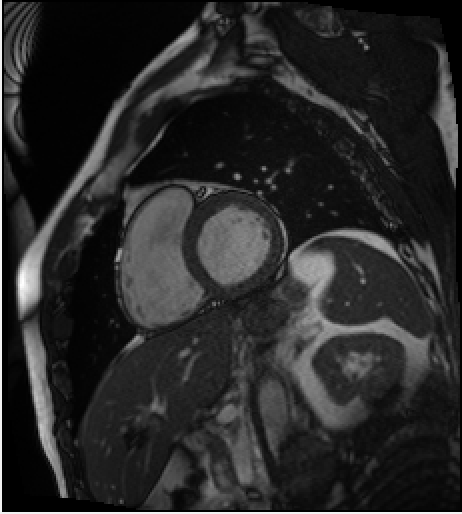
\includegraphics[width=150]{before.png}
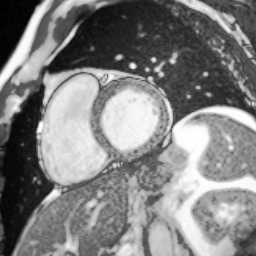
\includegraphics[width=150]{after.png}

Cele dou\u{a} imagini de mai sus reprezint\u{a} un exempu de imagine din setul de date \^{i}nainte de a fi procesat\u{a} \c{s}i dup\u{a} ce a fost procesat\u{a}, cum se poate observa imaginea procesat\u{a} a fost decupat\u{a} din mijlocul imaginii neprocesate astfel \^{i}nc\^{a}t s\u{a} se elimine o cantitate c\^{a}t mai mare de date care nu sunt necesare pentru scopul nostru, de asemenea se mai poate observa c\u{a} imaginea procesat\u{a} are un contrast mai mare fa\c{t}\u{a} de imaginea neprocesat\u{a} iar detaliile imaginii se pot observa mai bine, aceste lucruri vor duce la o vitez\u{a} de calcul \c{s}i la o acurate\c{t}e mai mare a re\c{t}elei neuronale.